\section{Rate Distortion Theory}
Rate Distortion Encoder and Decoder:
\begin{figure}[htbp]
    \centering
    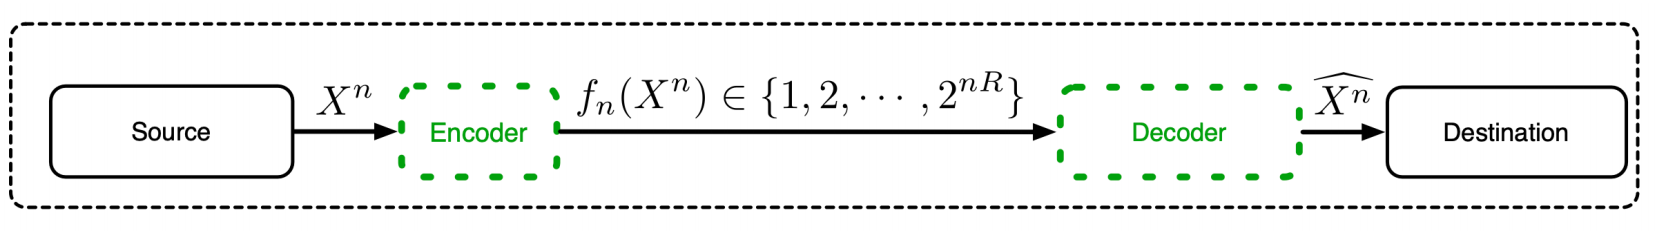
\includegraphics[width=\textwidth]{./figures/chapter8/rate_distortion.png}
\end{figure}

Rate-distortion theory describes the trade-off between lossy compression rate and the resulting distortion. \\
Lossless Source coding: Recover source data X without error \\
Lossy source coding: Recover source with some error and distortion

\begin{figure}[htbp]
    \centering
    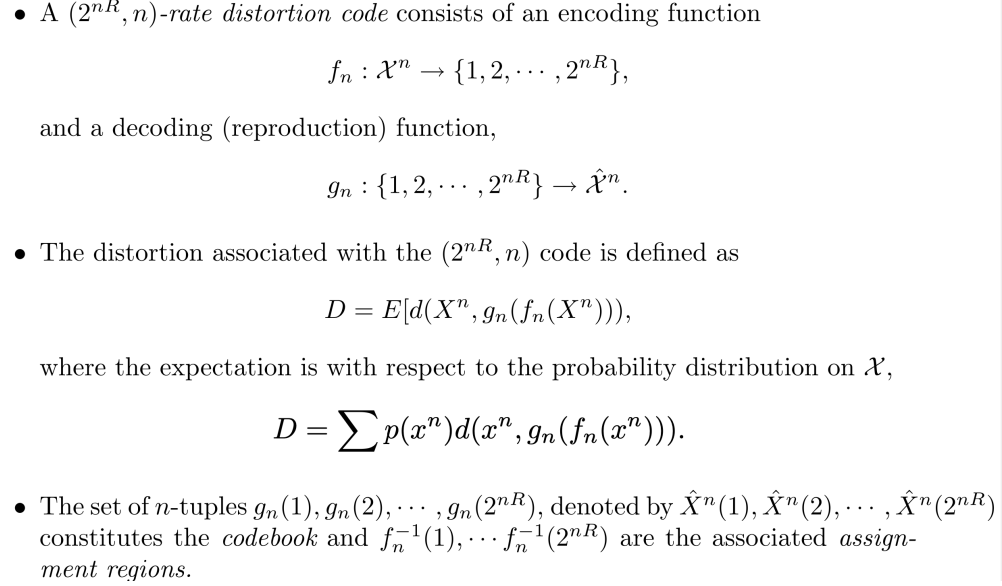
\includegraphics[width=\textwidth]{./figures/chapter8/definition.png}
\end{figure}
其中$f$是Encoder, $g$是Decoder, $g_n\left(f_n(X^n)\right)$即为$\hat{X}^n$. \\
$f^{-1}_n(1),\ldots,f^{-1}_n(2^{nR})$: 一个区域量化成一个值. \\
$D$: distortion上界, $R$: 压缩速率 (每个symbol用$R$ bit表示). \\
$D=0\Rightarrow$ 无损压缩(Lossless compression), $R=H(X)\Rightarrow$ 达到压缩极限. \\
$D$越大, $R$越小: 允许的误差越大, 就可以用更少的bit进行压缩, 所以压缩速率可以写作$R(D)$.

\newpage

\begin{figure}[htbp]
    \centering
    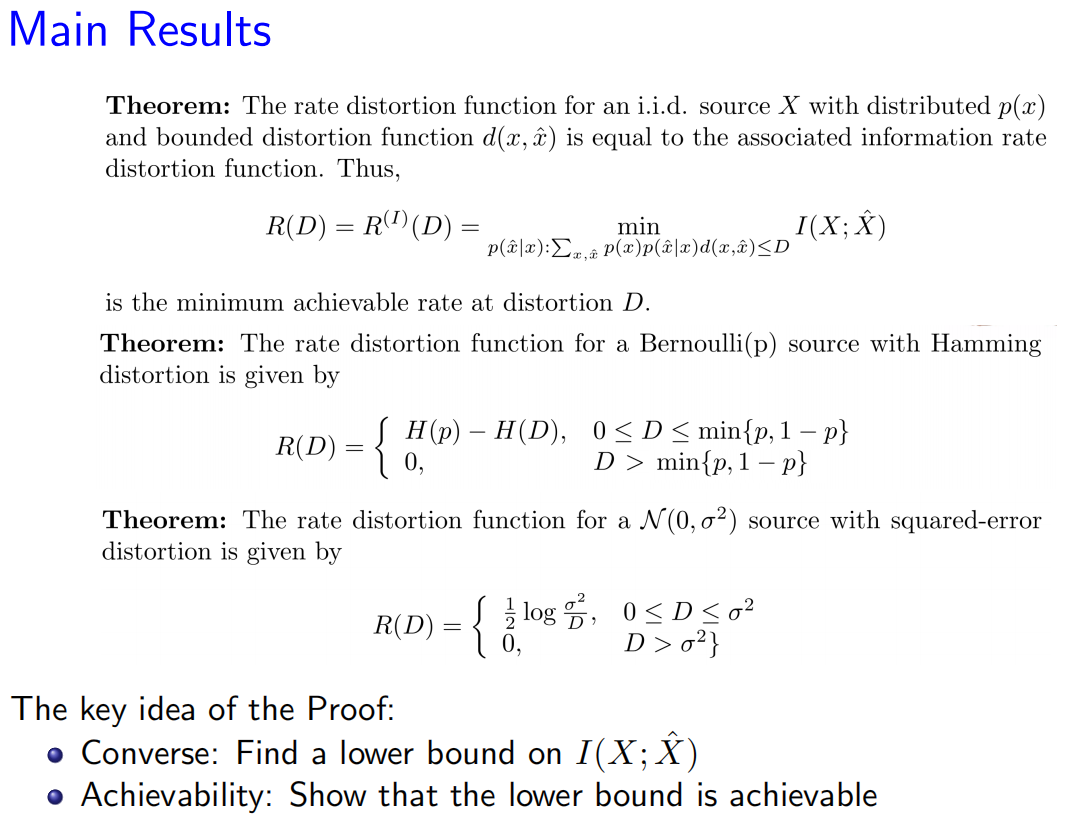
\includegraphics[width=\textwidth]{./figures/chapter8/result.png}
\end{figure}
这里 W.L.O.G, $p\leq \dfrac{1}{2}$. \\
$R(D)=0$: 所有symbol都压缩成一个constant $\Rightarrow D$太大了, 盲猜都能使得distortion小于$D$. \\
"For a $\mathcal{N}(0,1)$ source": 假设的信源分布. \\
$X\sim Bern\left(p\right)\Rightarrow G(D)=H(X)=H(p)$. \\
$R(D)=\dfrac{1}{2}\log\left(\dfrac{\sigma^2}{D}\right)\Rightarrow D=\sigma^2 2^{-2R}$.

Some notes: \\
Given $p(x)$, $I(X;\hat{X})$ 关于 $p(\hat{x}|x)$ convcave. \\
$(\tilde{x}, \tilde{y})\sim p(x)p(y)\Rightarrow \Pr\left[(\tilde{x}, \tilde{y})\in A_{\epsilon}^{(n)}(P_{X,Y})\right] \to 2^{-nI(X;Y)}$.

Other details see in ppt.